\chapter{Theoretical framework}


\section{The mathematical model} \label{sec:modelo}

To describe the thermoluminescent response of a semicoductor, we can use a mathematical model based on the trapping and releasing of charge carriers in the accesible energy levels of the material. 

\vspace{10pt}

Let us first consider the case of an arbitrary semicoductor without impurities. The energy levels of the conduction band and the valence band are separated by a bandgap $E_g$, and can be obtained with Schrodinger's equation that is under the influence of a periodic potential:

\begin{equation} \label{eq:schrodinger}
  \left[ -\frac{\hbar^2}{2m} \nabla^2 + V(\vec{r}) \right] \psi(\vec{r}) = E ~ \psi(\vec{r}),
\end{equation}

\vspace{10pt}
The periodicity of the potential $V(\vec{r})$ for any lattice vector $\vec{R}$ allows the Bloch's theorem to apply, and so it gives rise to the formation of a band structure, composed by the conduction band, which is typically fully occupied at absolute zero temperature, and the valence band, which is in turn typically empty -or rather, we can consider it filled with holes ($h^+$), or ``positively charged electrons''. The bandgap $E_g$ is then defined as the energy difference between the top of the valence band and the bottom of the conduction band, and for a perfect crystal, no energy states are allowed in that region. This can be clearly seen if we take into account the density of available states, $D(E)$, which is a function of the Fermi-Dirac distribution $f(E)$ for a certain temperature $T$. This function gives the occupancy of any energy level $E$, and can be expressed as:

\begin{equation} \label{eq:fermidirac}
  f(E) = \frac{1}{e^{\frac{E - E_f}{k_B T}} + 1},
\end{equation}

\vspace{10pt}
Where $E_f$ is the Fermi Level, and $k_B$ is the Boltzmann constant. If the system is in equilibrium, and we set the case of $T=0K$, the occupancy function $f(E)$ will be equal to 1 for all energy levels below the Fermi level, and 0 for all energy levels above it. This means that the occupancy function will be a step function, with a discontinuity at the Fermi level, and so we can see that there are no available states in the bandgap region.

\begin{figure}[H]
  \centering
  
\includegraphics[width=0.9\textwidth]{Images/FD_irradiation.png}
  \caption{Fermi-Dirac distribution for a semicoductor that is irradiated.}
  \label{fig:FD_irradiation}
\end{figure}


\vspace{10pt}
The introduction of impurities or defects however, break the periodicity of the lattice, and create localized energy levels inside this ``forbidden region''. These levels can be thought of as traps for electrons if we are situated above the fermi level, and traps of holes if we are situated below. When this material is irradiated, electrons from the valence band can be excited to the conduction band, creating an electron-hole pair; and so changing the shape of the occupancy function. Once excited, both electrons and holes get ``trapped'' in these localized energy levels, and the excitation of these pairs into equilibrium will result in the emission of energy. In Figure \ref{fig:FD_irradiation} we can see a broad description of the perturbation of the system from its equilibrium state due to the irradiation, and the return of the system to equilibrium during either thermal stimulation or optical stimulation. If said relaxation processes are radiative, TL and OSL result. 

\begin{figure}[H]
  \centering
  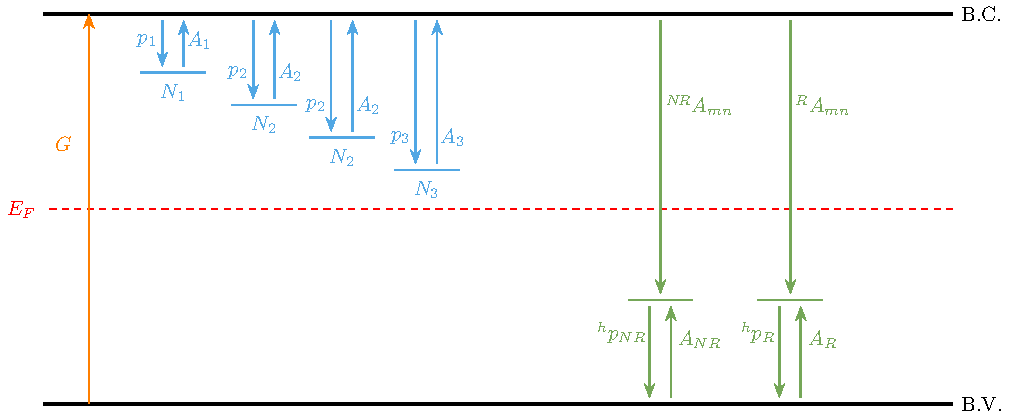
\includegraphics[width=0.8\textwidth]{Images/modeldiagram.pdf}
  \caption{Schematic representation of the theoretical model.}
  \label{fig:TheoreticalModel}
\end{figure}

And so, we can see a schematic representation of our theoretical model in Figure \ref{fig:TheoreticalModel}. Situating the energy in the Y axis, the focus is set in the energy gap of our material. Drawn as a blue or green horizontal line are the energy traps; in blue above the Fermi level there are electron traps, and in green there are hole traps or recombination centers. The vertical arrows describe available transitions; the ones pointing upwards represent an excitation process, and the ones pointing downwards represent a relaxation process. 

\vspace{10pt}

Mathematically, we can describe these processes with a set of differential equations that take into account the rate of change of the number of electrons and holes in the bands and traps. This set will depend on the properties of the material, and the luminescence response we are trying to model. For an arbitrary system, we can write the following set of equations that describe the rate of change of the number of electrons and holes in the conduction band $n_c$, the valence band $n_v$:
\vspace{10pt}

\begin{equation} \label{eq:dn_cdt}
  \frac{dn_c}{dt} = \textcolor{orange}{G} - \textcolor{customblue}{\left[\sum_i \frac{dn_i}{dt}\right]} \cdot n_c - \textcolor{customgreen}{\left[ \sum_{j=R, N\!R}\, ^iA_{mn} \cdot m_j \right]} \cdot n_c
\end{equation}

\begin{equation} \label{eq:dn_idt}
  \textcolor{customblue}{\frac{dn_i}{dt} = -p_i \cdot n_i + A_i \cdot [N_i - n_i]}
\end{equation}

\begin{equation} \label{eq:dm_jdt}
  \textcolor{customgreen}{\frac{dm_j}{dt} = -^hp_j \cdot m_j + A_j \cdot [M_j - m_j]} \cdot n_v - \textcolor{customgreen}{^iA_{mn} \cdot m_j} \cdot n_c
\end{equation}

\begin{equation} \label{eq:dn_vdt}
  \frac{dn_v}{dt} = \textcolor{orange}{G} - \textcolor{customgreen}{\sum_{j=R, N\!R} \left[-^hp_j \cdot m_j + A_j \cdot [M_j - mj] \textcolor{black}{~ \cdot ~n_v}\right]} 
\end{equation}

\vspace{15pt}
Where every term is defined as follows:
\begin{itemize}[itemsep=0.2cm,parsep=0cm]
  \item $G$: electron-hole pairs generated by the radiation [cm$^{-3}$ s$^{-1}$]
  \item $n_c$: electron density in the conduction band [cm$^{-3}$]
  \item $n_v$: electron density in the valence band [cm$^{-3}$]
  \item $n_i$: electron density in trap i [cm$^{-3}$]
  \item $m_j$: hole density in the recombination center j [cm$^{-3}$]
  \item $N_i$: total density of ???
  \item $M_j$: total density of ???
  \item $p_i$: electron release probability factor for trap i [s$^{-1}$]
  \item $^hp_j$: hole release probability factor for recombination center j [s$^{-1}$]
  \item $A_i$: electron trapping probability factor for trap i [cm$^{3}$ s$^{-1}$]
  \item $^iA_{mn}$: recombination probability factor for recombination center j [cm$^{3}$ s$^{-1}$]
\end{itemize}

\vspace{10pt}

Equation \ref{eq:dn_cdt} describes the change rate of electron concentrations in the conduction band. To interpret this equation, we can see that to the electron-hole pairs generated by the radiation ($G$), there are two terms substracted. The first one correlates to the electrons that leave the continuum levels of the conduction band and get trapped in the discrete levels of the material ---a process described by \ref{eq:dn_idt}, that will have a further discussion in section \ref{sec:factorfrecuencia}---, and the second one answers to the electrons in the conduction band that recombine with holes with a radiative ($R$) or non-radiative ($N\!R$) process. It is easy to see that this second term corresponds to the third term of \ref{eq:dm_jdt}. 

\vspace{10pt}
The change rate of electron concentrations in the valence band is shown in \ref{eq:dn_vdt}, and it follows a similar logic. This time however, we only take into account the terms multiplied by the electron density in the valence band ($n_v$) seen in equation \ref{eq:dm_jdt}; one that represents the holes leaving the continuum to get trapped in the recombination centers, and another that accounts for the addition of electrons that are released from the recombination centers and recombine with the holes in the valence band. The terms described correspond to Equations \ref{eq:dn_idt} and \ref{eq:dm_jdt} describe the total change rate of electrons and holes in the discrete levels of the material. The signs of the terms in these equations follow the convention that we are set in the conduction band, and so any electron that leaves the conduction band is represented with a negative term, and any electron that enters is represented with a positive term.

\vspace{10pt}
Luminescence results when the electrons and holes recombine, so its intensity will be proportional to the number of recombinations that occur, given by equation \ref{eq:dm_jdt} \cite{mckeever_course_2022}. Assuming that after irradiation there is no further hole trapping, the luminescence intensity ($I$) can be expressed as:

\begin{equation} \label{eq:intensity}
  I(t) \approx {}^RA_{mn} \cdot m_R \cdot n_c
\end{equation}

\vspace{10pt}
Representing this intensity as a function of time will be the objective of the simulations, as it is the key to understand the thermoluminescent response of the $LiF:M\!g,Ti$ after being irradiated.




\section{The frequency factor} \label{sec:factorfrecuencia}

As introduced in Section \ref{sec:modelo}, there is a greater discussion to be had about the releasing probability of electrons and holes, as it determines in great part the electron-hole pairs available to recombine. If we consider that after being irradiated, the material will release its carriers through \textit{thermal excitation}, an electron trapped in a lattice defect with energy $E_t$ and temperature $T$ will have a probability of being released that follows Arrhenius equation. The probability per second that the electron will be thermally excited into the conduction band is given by:

\begin{equation}
  p = s \cdot e^{-\frac{E_t}{k_B T}}
\end{equation}

\vspace{10pt}
Where $s$ is known as the \textit{frequency factor}. It can be interpreted as the ``attempt to escape'' frequency, as it is a measure of the number of times per second that energy is absorbed from phonons in the lattice. The exponential that follows is the probability that the energy absorbed is enough to cause a transition from the localized state to the conduction band. 

\vspace{10pt}

The frequency factor is a very important parameter in the study of thermoluminescence, as it determines the rate at which electrons are released from traps. It is a function of the material properties, as shown in its definition:

\begin{equation}
  s = \nu \cdot K \cdot e^{\frac{\Delta S}{k_B}}
\end{equation}

\vspace{10pt}
Where $\nu$ is the lattice phonon vibration frequency and $K$ is the transition probability constant. Typically, one can expect $s \sim 10^{12} -10^{14}$ s$^{-1}$, which is consistent with the values of $\nu$ for most solids. The term $e^{\frac{\Delta S}{k_B}}$ is a correction factor that accounts for the entropy change associated with the transition from the localized state to the conduction band. 





















\section{About LiF:Mg,Ti} \label{sec:LiF}


Lithium fluoride (LiF) is a crystalline material that has been widely used in radiation dosimetry due to its favorable % !!!!
properties. It first appeared as a thermoluminescent dosimetry material in the 1950's, and since then, it has been extensively studied in the field of radiation detection. The material is composed of lithium (Li) and fluor (F) %?????
atoms, forming a crystal lattice structure of a face-centered cubic (FCC) type. Without any impurities, LiF is a semiconductor, with a bandgap of approximately 14 eV, which makes it an excellent insulator at room temperature.

\vspace{10pt}

To enhance the properties for radiation detection, LiF is often doped with magnesium (Mg) and titanium (Ti) ions, and sold commercially as TLD-100 \cite{lif}. The doping process introduces defects in the crystal lattice, creating energy levels within the bandgap. These defects play a crucial role in trapping and releasing charge carriers, which are responsible for the thermoluminescent response of the material. This process is known as thermoluminescence (TL), where the trapped electrons are released upon heating, resulting in the emission of light. The intensity of this emitted light is proportional to the amount of radiation absorbed by the material, making it a valuable tool for dosimetry.